%!TEX root=../document.tex
\section{Projektaufbau}
\begin{minipage}{\linewidth}
	\centering
	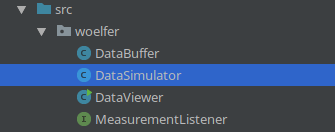
\includegraphics[width=0.5\linewidth]{images/projekt}
\end{minipage}

Die Klassen \verb|Databuffer|, \verb|DataSimulator| und \verb|MeasurementListener| wurden bereits vorgegeben.

\subsection{MeasurementListener}
Das \textbf{Interface} definiert die Methode, welche aufgerufen wird sobald eine neue \textbf{Messung} eintrifft, \verb|measurementReceived()| 

Dieser wird im \verb|DataBuffer| mit der Methode \verb|addMeasurementListener| hinzugefügt. 

Wenn nun die Methode \verb|addList()| vom Buffer aufgerufen wird, wird automatisch \verb|measurementReceived()| des Listeners aufgerufen.

\subsection{DataBuffer}
Diese Klasse würde in einem klassischen \textbf{MVC-Modell} das \textbf{Model} darstellen. Der \verb|DataBuffer| hält die Liste, für die Werte welche simuliert werden. Der Buffer bestimmt auch die Anzahl der ausgerechneten Werte mit der Konstante \verb|SIZE|.

\subsubsection{addList}
Diese Methode ''überschreibt'' die momentane Liste der Werte, und ersetzt mit jener welche übergeben wird als Parameter. Zusätzlich wird noch die \verb|measurementReceived()| Methode des Listeners aufgerufen.

\subsubsection{getNext}
Diese Methode kopiert das momentane Array mit allen Werten, und übergibt es an die Variable welcher übergeben wird - auch \textbf{Callback-Variable} genannt. 

Der Grund dafür, dass die Liste nicht einfach \textbf{return}ed wird sondern \textbf{kopiert}, liegt darin dass Konflikte entstehen könnten, da der \verb|DataSimulator|, als Thread,  immer parallel läuft und Zugriffsprobleme entstehen könnten, da der Simulator auch auf die Liste zugreift.



\subsection{DataSimulator}
Der \verb|DataSimulator| stellt einen Thread dar. Deswegen erweitert diese Klasse die Klasse \verb|Thread| und \textbf{überschreibt} die \verb|run()| Methode des Threads.

Diese Klasse übernimmt folgende Parameter, um Eigenschaften der Sinuskurve zu definieren:

\begin{itemize}
	\item minFrequency (Standard: 0.5)
	\item maxFrequency (Standard: 5)
	\item deltaFrequency (Standard: 0.015)
\end{itemize}

Der Simulator nimmt zusätzlich noch eine Instanz vom Typen \verb|DataBuffer|, in welcher er die simulierten Daten ''speichert''.

\subsubsection{run}
Wie schon erwähnt, liegt die gesamte Logik in der run Methode, da diese parallel zu den anderen Prozessen laufen kann.

Es wird nun eine \verb|values| Liste angelegt, in welcher die Werte für eine Sinuskurve gespeichert werden. Wenn die Berechnung vollständig durchgeführt wurde und die vorübergehende Liste gefüllt ist, wird die Liste der DataBuffer-Instanz gesetzt.

Anschließend wird die Frequenz verändert, damit bei der Visualisierung eine sich änderte Sinuskurve zu sehen ist. Danach wiederholt sich alles da der gesamte Block mit einer While-true Schleife umschlossen ist.

\clearpage

\subsection{DataViewer}
Die Klasse \verb|DataViewer| stellt ein \verb|JComponent| dar, welches in ein \verb|JFrame| gepackt wird um gezeichnet zu werden.

\subsubsection{main}
\begin{lstlisting}[language=Java]
public static void main(String[] args){
	frame = new JFrame("DataViewer");
	frame.setDefaultCloseOperation(WindowConstants.EXIT_ON_CLOSE);
	frame.getContentPane().add(new DataViewer());
	frame.pack();
	frame.setSize(new Dimension(800, 400));
	frame.setVisible(true);
}
\end{lstlisting}
In der main-Methode, wird wie bereits erwähnt, ein JFrame erzeugt in welches, mit der Methode \verb|frame.getContentPane().add()| das JComponent, also der \verb|DataViewer|, hinzugefügt. 

Anschließend werden noch Dimensionen und obligatorische JFrame Methoden gesetzt.

\subsubsection{constructor}
Zuerst wird ein \verb|DataBuffer| Objekt erzeugt, welches anschließend mit zusätzlichen Parametern an den Simulator übergeben wird um diesen zu starten. Es wird auch eine die Liste \verb|yPoints| erzeugt, welche die Werte des Simulators halten wird.

Ein wichtiger Schritt ist es, dem DataBuffer nun per \verb|addMeasurementListener| einen \verb|MeasurementListener| hinzuzufügen.

Um den Code einfacher darzustellen, wurde gleich in der Instanziierung definiert, was passieren soll wenn eine neue Messung erhalten wurde. Es soll nun die yPoints Liste gesetzt werden mit \verb|next()| des Buffers, und das frame \verb|repaint|ed werden, damit die Sinuskurve sich bei einer neuen Messung tatsächlich aktualisiert:

\begin{lstlisting}[language=Java]
DataBuffer db = new DataBuffer();
yPoints = new int[DataBuffer.SIZE];
DataSimulator dt = new DataSimulator(0.5, 5, 0.015, db);
db.addMeasurementListener(new MeasurementListener(){
	@Override
	public void measurementReceived() {
		db.getNext(yPoints);
		frame.repaint();
	}
});
\end{lstlisting}

\subsubsection{paint}
Diese Methode wird von \verb|JComponent| vererbt. Durch überschreiben dieser Methode, kann definiert werden was gezeichnet werden soll wenn die Komponente geladen wird. Um die Sinuskurve zu simulieren, wird das Package \verb|GeneralPath| verwendet. Damit ist es möglich, Linien von einem Punkt zu einem anderen zu zeichnen. 

Die Idee ist, da sehr viele Werte geliefert werden vom Simulator, zwischen jedem dieser Werte einen Strich zu ziehen um somit den Anschein, eine echte Sinuskurve zu zeichnen, zu erwecken.

Zuerst wird eine path Instanz erzeugt, und zum Mittelpunkt des Fenster navigiert:

\begin{lstlisting}[language=Java]
GeneralPath path = new GeneralPath(GeneralPath.WIND_EVEN_ODD, DataBuffer.SIZE);

path.moveTo(0, frame.getHeight() / 2);
\end{lstlisting}

\begin{lstlisting}[language=Java]
for (int i = 0; i < DataBuffer.SIZE; i++){
	path.lineTo(i*10, (yPoints[i]/70)+(this.frame.getHeight()/2));
}
\end{lstlisting}

In diesen Zeilen werden die einzelnen Linien dem Path hinzugefügt.

Die Methode \verb|lineTo| nimmt 2 Punkte als Parameter. Es ist sich vorzustellen, der erste Punkt sei der Punkt auf der ''x-Achse'' und der zweite die Auswertung der ''y-Achse''. Wie bereits erwähnt, werden in \verb|yPoints| die Werte des Simulators gespeichert.

Diese werden durch eine Konstante dividiert, um die Werte der Fenstergröße anzupassen, und um die Hälfte des Fenster nach unten geschoben damit die Kurve in der Mitte liegt.

Zum Schluss wird noch ein \verb|Graphics2D| Objekt erzeugt, mit welchem tatsächlich der path gezeichnet wird:

\begin{lstlisting}[language=Java]
Graphics2D g2 = (Graphics2D) g;
g2.draw(path);
\end{lstlisting}

\section{Ergebnis}
\begin{minipage}{\linewidth}
	\centering
	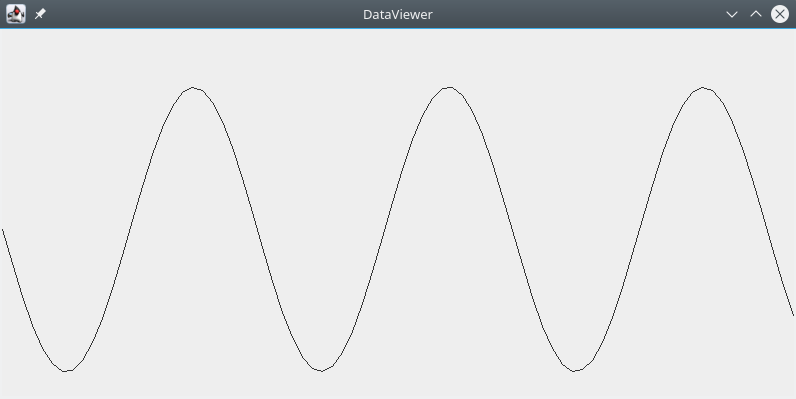
\includegraphics[width=1\linewidth]{images/ss}
	\figcaption{Sinuskurve wird simuliert in Java}
\end{minipage}
